\chapter{Optymalizacja: jak sieć się uczy}\label{rozdz:optymalizacja}

\section{Od gradientu do działającego uczenia}

W rozdziale~\ref{rozdz:pochodne} poznaliśmy spadek gradientu $\vect\theta\leftarrow\vect\theta-\eta\nabla L$. W praktyce potrzeba czterech poprawek: (i)~gradient liczymy z \emph{małej porcji} danych, nie ze wszystkich (SGD), (ii)~dostosowujemy krok do każdego parametru osobno (Adam),
(iii)~dodajemy zanik wag, (iv)~zmieniamy krok $\eta$ w czasie (harmonogram). Ten rozdział uzasadnia każdy z tych kroków i podaje wartości użyte w Gen~6.

Po tym rozdziale umiesz: (i)~wskazać największy bezpieczny krok uczenia dla paraboli, (ii)~policzyć krok Adama, (iii)~obliczyć wartość kroku w dowolnej chwili harmonogramu z rozgrzewką i kosinusem, (iv)~uzasadnić przycinanie gradientu.

\section{Kiedy spadek gradientu się zbiega?}

\begin{twierdzenie}[Kryterium stabilności]\label{tw:eta}
Dla $L(\vect x)=\tfrac12\sum_{i}\lambda_ix_i^2$ z $\lambda_i>0$ spadek gradientu z krokiem $\eta$ daje $x_i^{(k)}=(1-\eta\lambda_i)^kx_i^{(0)}$. Zbiega on do zera dla każdej współrzędnej wtedy i tylko wtedy, gdy
$\eta<2/\lambda_{\max}$. Najszybszy zbieżny wybór to $\eta^\ast=\dfrac{2}{\lambda_{\min}+\lambda_{\max}}$, z współczynnikiem $\rho=\dfrac{\lambda_{\max}-\lambda_{\min}}{\lambda_{\max}+\lambda_{\min}}$ na krok.
\end{twierdzenie}
\begin{pomyslDowodu}
Funkcja jest rozdzielona po współrzędnych, więc każda ewoluuje osobno jak ciąg geometryczny o ilorazie $1-\eta\lambda_i$; ciąg zbiega do zera, gdy $|1-\eta\lambda_i|<1$.
\end{pomyslDowodu}
\begin{proof}
$\partial L/\partial x_i=\lambda_ix_i$, więc
\begin{align*}
x_i^{(k+1)} &= x_i^{(k)}-\eta\lambda_ix_i^{(k)} && \pow{(def.~\ref{def:spadek})}\\
 &= (1-\eta\lambda_i)\,x_i^{(k)}. && \pow{(wyłączenie)}
\end{align*}
Z indukcji $x_i^{(k)}=(1-\eta\lambda_i)^kx_i^{(0)}$. Ciąg geometryczny zbiega do $0$ dla dowolnej wartości początkowej wtedy i tylko wtedy, gdy $|1-\eta\lambda_i|<1$, czyli $0<\eta\lambda_i<2$.
Warunek dla wszystkich $i$ jednocześnie to $\eta<2/\lambda_{\max}$ (najostrzejszy). Tempo ogranicza współrzędna z największym $|1-\eta\lambda_i|$, czyli $\rho(\eta)=\max\big(|1-\eta\lambda_{\min}|,|1-\eta\lambda_{\max}|\big)$.
Pierwszy argument maleje z $\eta$, drugi (dla $\eta>1/\lambda_{\max}$) rośnie; przecinają się, gdy $1-\eta\lambda_{\min}=\eta\lambda_{\max}-1$, czyli $\eta^\ast=2/(\lambda_{\min}+\lambda_{\max})$, a wtedy $\rho=1-\eta^\ast\lambda_{\min}=(\lambda_{\max}-\lambda_{\min})/(\lambda_{\max}+\lambda_{\min})$. To kończy dowód.
\end{proof}

W zwykłym języku: najbardziej „stromy” kierunek (największe $\lambda$) ogranicza krok dla całej doliny, a najbardziej płaski (najmniejsze $\lambda$) ogranicza tempo. Im bardziej wydłużona dolina ($\lambda_{\max}/\lambda_{\min}$ duże), tym wolniej schodzimy.

\begin{naliczbach}
Dolina z rozdziału~\ref{rozdz:pochodne}: $\lambda=(1,10)$. Granica kroku: $2/10=0{,}2$. Dla $\eta=0{,}19$ współrzędna $y$ mnoży się przez $1-1{,}9=-0{,}9$ w każdym kroku: zbieżna, ale z drżeniem. Dla $\eta=0{,}21$: $1-2{,}1=-1{,}1$ --- błąd rośnie $10\%$ na krok i metoda się rozbiega.
Najlepszy krok $\eta^\ast=2/11=0{,}182$ daje $\rho=9/11=0{,}818$: żeby zmniejszyć błąd $1000$-krotnie, potrzeba $\ln10^{-3}/\ln0{,}818\approx34$ kroków (rys.~\ref{rys:optymalizacja}a).
\end{naliczbach}

\begin{intuicja}
Wyobraź sobie kulkę w długim, wąskim korycie. Gradient w poprzek koryta jest ogromny, a wzdłuż niego malutki, więc zwykły spadek gradientu musi używać małego kroku (bezpiecznego dla ściany) i wolno posuwa się wzdłuż koryta.
Adam dzieli ruch w każdej osi przez jej typową skalę gradientu, dzięki czemu obie osie robią krok podobnej wielkości \emph{bez ręcznego dobierania $\eta$ do skali każdego parametru}.
Uczciwie trzeba dodać: na prostej paraboli z \emph{idealnie} dobranym krokiem zwykły spadek gradientu jest lepszy (rys.~\ref{rys:adam-dolina}); zaleta Adama ujawnia się w sieciach, gdzie skale gradientów różnią się między warstwami o wiele rzędów wielkości i jednego dobrego $\eta$ nie da się wybrać.
\end{intuicja}

\begin{figure}[ht]
\centering
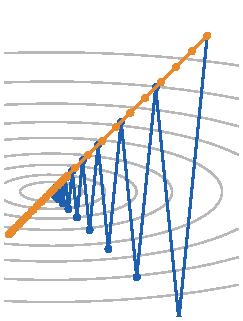
\includegraphics[width=\linewidth]{figures/adam-dolina.pdf}
\sidecaption{Ta sama dolina $L=\frac12(x^2+10y^2)$ co w rozdziale~\ref{rozdz:pochodne}, start $(1,1)$, $40$ kroków. Niebieska: spadek gradientu z optymalnym krokiem $2/11$ (strata końcowa $6\cdot10^{-7}$).
Pomarańczowa: Adam z $\eta=0{,}1$ (strata końcowa $0{,}056$: długie kroki w obu osiach, ale potem drży wokół minimum). Szare warstwice to poziomy strat. Na tej prostej paraboli, przy idealnie dobranym kroku, wygrywa zwykły spadek gradientu. Obie ścieżki obliczone programem. \label{rys:adam-dolina}}
\end{figure}

\section{SGD i jego szum}

Strata całego zbioru to średnia strat pojedynczych próbek: $L(\vect\theta)=\frac1N\sum_{n}\ell_n(\vect\theta)$. Liczenie jej gradientu dla $N=15\,600$ nagrań w każdym kroku byłoby za drogie, więc losujemy \emph{paczkę} $B$ i bierzemy
$\hat g=\frac1{|B|}\sum_{n\in B}\nabla\ell_n$.

\begin{twierdzenie}[Gradient z paczki jest nieobciążony]\label{tw:sgd}
Jeśli $B$ składa się z $|B|$ próbek wylosowanych niezależnie i równomiernie z $\{1,\dots,N\}$, to $\Exp[\hat g]=\nabla L(\vect\theta)$.
\end{twierdzenie}
\begin{pomyslDowodu}
Każda próbka trafia do paczki z prawdopodobieństwem $\frac1N$; wartość oczekiwana średniej to średnia wartości oczekiwanych.
\end{pomyslDowodu}
\begin{proof}
\begin{align*}
\Exp[\hat g] &= \frac1{|B|}\sum_{j=1}^{|B|}\Exp\big[\nabla\ell_{n_j}\big] && \pow{(liniowość $\Exp$)}\\
 &= \frac1{|B|}\sum_{j=1}^{|B|}\sum_{n=1}^{N}\frac1N\nabla\ell_n && \pow{($n_j$ jednostajne)}\\
 &= \frac1N\sum_{n=1}^N\nabla\ell_n=\nabla L(\vect\theta). && \pow{($|B|$ jednakowych składników)}
\end{align*}
Gradient z paczki jest więc szumem wokół prawdziwego, ze średnią równą prawdziwemu; jego wariancja maleje jak $1/|B|$. To kończy dowód.
\end{proof}

W Gen~6 paczka to $16$ losowych wycinków po $192$ klatki ($4{,}4$ s); wycinki są losowane z trzech źródeł z prawdopodobieństwami $0{,}5$ (klasyka), $0{,}3$ (GuitarSet) i $0{,}2$ (środowiska).

\section{Adam i AdamW}

W różnych częściach sieci gradienty mają bardzo różną skalę. \emph{Adam} utrzymuje dla każdego parametru wygładzoną średnią gradientu $m$ i wygładzoną średnią jego kwadratu $v$:
\begin{align*}
m_t &= \beta_1m_{t-1}+(1-\beta_1)g_t, & v_t &= \beta_2v_{t-1}+(1-\beta_2)g_t^2,\\
\hat m_t &= \frac{m_t}{1-\beta_1^t}, & \hat v_t &= \frac{v_t}{1-\beta_2^t},\\
\theta_t &= \theta_{t-1}-\eta\Big(\frac{\hat m_t}{\sqrt{\hat v_t}+\varepsilon}+\lambda\theta_{t-1}\Big),
\end{align*}
z $m_0=v_0=0$, zwykle $\beta_1=0{,}9$, $\beta_2=0{,}999$, $\varepsilon=10^{-8}$. Człon $\lambda\theta$ to \emph{zanik wag} (w AdamW dodawany osobno; Gen~6: $\lambda=10^{-4}$), który delikatnie ściąga wagi do zera i ogranicza przeuczenie.

\begin{twierdzenie}[Korekta obciążenia i niezmienniczość skali]\label{tw:adam}
(a) Jeśli $g_t=g$ jest stałe, to $m_t=(1-\beta_1^t)g$, więc $\hat m_t=g$. (b) Jeśli pomnożymy wszystkie gradienty przez $c>0$, to przy $\varepsilon\to0$ krok Adama się nie zmienia.
\end{twierdzenie}
\begin{pomyslDowodu}
(a) Indukcja po $t$; (b) $\hat m$ rośnie $c$ razy, a $\sqrt{\hat v}$ też $c$ razy; czynnik się skraca.
\end{pomyslDowodu}
\begin{proof}
(a) Dla $t=1$: $m_1=(1-\beta_1)g=(1-\beta_1^1)g$. Jeśli $m_{t-1}=(1-\beta_1^{t-1})g$, to
\begin{align*}
m_t &= \beta_1(1-\beta_1^{t-1})g+(1-\beta_1)g && \pow{(założenie indukcyjne)}\\
 &= (\beta_1-\beta_1^t+1-\beta_1)g=(1-\beta_1^t)g. && \pow{(redukcja)}
\end{align*}
Dzielenie przez $1-\beta_1^t$ daje $\hat m_t=g$. Bez korekty pierwsze kroki byłyby $1-\beta_1=10\%$ właściwej wartości.
(b) $\hat m\mapsto c\hat m$ (liniowość), $\hat v\mapsto c^2\hat v$, $\sqrt{\hat v}\mapsto c\sqrt{\hat v}$, więc $\hat m/\sqrt{\hat v}$ się nie zmienia. To kończy dowód.
\end{proof}

\begin{przyklad}[Pierwszy krok Adama]\label{prz:adam}
Dla $t=1$: $\hat m_1=g_1$ i $\hat v_1=g_1^2$, więc krok to $\eta g_1/|g_1|=\eta\,\mathrm{sgn}(g_1)$ ($\varepsilon\to0$). Dla gradientów $(0{,}001;\ 100)$ oba parametry zmienią się o dokładnie $\eta=10^{-3}$. Zwykły SGD zmieniłby je o $10^{-6}$ i $0{,}1$, czyli o liczby różniące się pięć rzędów wielkości.
\end{przyklad}

\haslo{przycinanie gradientu}
\begin{definicja}[Przycinanie gradientu]\label{def:clip-grad}
Zamiast $g$ używamy $g\cdot\min(1,\,c/\norm{g})$ (norma po wszystkich parametrach). Dla $\norm g\le c$ nic się nie zmienia; dla większej normy kierunek zostaje, a długość spada do $c$.
\end{definicja}

\begin{przyklad}\label{prz:clip}
Dla $g=(3,4)$, $\norm g=5$, $c=1$: $g\cdot\min(1,0{,}2)=(0{,}6;\,0{,}8)$, długość $1$. Gen~6 przycina do $c=1$: pojedynczy dziwny wycinek nie wytrąci sieci z toru.
\end{przyklad}

\section{Harmonogram kroku}

Na początku uczenia wagi są losowe, a Adam ma jeszcze niedokładne $\hat v$ --- duży krok łatwo wszystko zepsuje; pod koniec chcemy kroku małego, by osiąść w dolinie. Stosujemy \emph{rozgrzewkę} (liniowy wzrost od $0$ do $\eta_0$ przez $W$ kroków) i potem \emph{spadek kosinusowy}:
\begin{equation}
  \eta(t)=\begin{cases}\eta_0\,\dfrac tW,& t<W,\\[2mm]\eta_0\cdot\tfrac12\big(1+\cos\pi q\big),\quad q=\dfrac{t-W}{T-W},& t\ge W.\end{cases}
\end{equation}

\begin{naliczbach}
Sesja~1 Gen~6: $\eta_0=10^{-3}$, $W=1000$, $T=36\,000$ (36 epok po 1000 kroków). Dla $t=500$: $\eta=5\cdot10^{-4}$. Dla $t=15\,000$ ($q=0{,}4$): $\eta=10^{-3}\cdot\tfrac12(1+\cos0{,}4\pi)=6{,}55\cdot10^{-4}$,
a dziennik uczenia zapisał na końcu epoki~14 wartość $6{,}55\cdot10^{-4}$. W połowie ($t=18\,500$, $q=0{,}5$): $5\cdot10^{-4}$. Na końcu $\eta\to0$.
\end{naliczbach}

\begin{figure*}[ht]
\centering
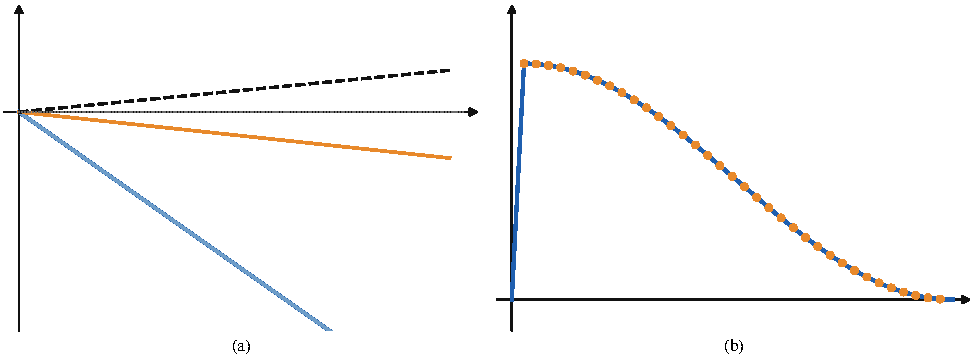
\includegraphics[width=\linewidth]{figures/optymalizacja.pdf}
\caption{(a) Spadek gradientu dla $\lambda=10$ ($\log_{10}|x|$ w kolejnych krokach): $\eta=0{,}05$ (niebieska) i $0{,}15$ (jasnoniebieska) zbiegają; $\eta=0{,}19$ (pomarańczowa) zbiega z wolno gasnącym drżeniem; $\eta=0{,}21>2/\lambda$ (czarna przerywana) rozbiega się. Szara kropkowana to poziom początkowy.
(b) Harmonogram kroku z rozgrzewką i spadkiem kosinusowym (niebieska) oraz wartości zapisane w dzienniku prawdziwego uczenia Gen~6 po każdej epoce (pomarańczowe kropki): leżą dokładnie na krzywej.}
\label{rys:optymalizacja}
\end{figure*}

W Gen~6 uczenie przebiegło w trzech sesjach (w sumie $97$ epok): sesja~1 z $\eta_0=10^{-3}$, sesja~3 (restart) z $4\cdot10^{-4}$, sesja~4 z $3\cdot10^{-4}$ i harmonogramem kosinusowym liczonym od \emph{czasu}, a nie od liczby kroków (żeby skończyć dokładnie w limicie GPU).

\begin{pulapka}
Ten sam model bez rozgrzewki lub z za dużym $\eta$ może się „rozjechać” w pierwszych setkach kroków i nigdy nie dojść do dobrego wyniku; objaw to strata, która nagle skacze do dużej wartości lub \texttt{NaN}. Warto zapisywać stan modelu po każdej epoce (Gen~6 tak robi) i umieć wznowić uczenie od zapisu.
\end{pulapka}

\section*{Podsumowanie}
\begin{itemize}
\item Spadek gradientu na paraboli zbiega, gdy $\eta<2/\lambda_{\max}$; tempo zależy od $\lambda_{\max}/\lambda_{\min}$ (tw.~\ref{tw:eta}).
\item Gradient z paczki jest nieobciążonym, zaszumionym oszacowaniem gradientu pełnego (tw.~\ref{tw:sgd}).
\item Adam normuje krok przez $\sqrt{\hat v}$: ma niezmienniczą skalę, a korekta obciążenia daje $\hat m=g$ dla stałego gradientu (tw.~\ref{tw:adam}). AdamW dodaje zanik wag $\lambda=10^{-4}$.
\item Przycinanie gradientu do normy $1$ chroni przed pojedynczymi dziwnymi paczkami.
\item Harmonogram: rozgrzewka $1000$ kroków, potem kosinus do zera; dziennik uczenia Gen~6 zgadza się ze wzorem.
\end{itemize}

\begin{sprawdz}
\begin{enumerate}
\item Dla $\lambda=(2,50)$ podaj granicę kroku i najlepszy krok $\eta^\ast$ oraz współczynnik $\rho$.
\item Policz pierwszy krok AdamW dla $\theta=0{,}5$, $g=-0{,}2$, $\eta=10^{-3}$, $\lambda=10^{-4}$ ($t=1$, $\varepsilon\to0$).
\item Oblicz $\eta(t)$ dla $\eta_0=3\cdot10^{-4}$, $W=1000$, $T=49\,000$, $t=25\,000$.
\item Pokaż, że przycinanie gradientu do normy $c$ nie zmienia jego kierunku.
\end{enumerate}
\end{sprawdz}

\subsection*{Rozwiązania}
\begin{enumerate}
\item Granica $2/50=0{,}04$; $\eta^\ast=2/52=0{,}0385$; $\rho=48/52=0{,}923$ (bardzo wolno: wydłużona dolina).
\item $\hat m/\sqrt{\hat v}=g/|g|=-1$, więc $\theta\leftarrow\theta-\eta\big(-1+\lambda\theta\big)=0{,}5-10^{-3}(-1+0{,}5\cdot10^{-4})=0{,}5+10^{-3}\cdot0{,}99995=0{,}50099995$.
\item $q=(25\,000-1000)/48\,000=0{,}5$, więc $\eta=3\cdot10^{-4}\cdot\tfrac12(1+0)=1{,}5\cdot10^{-4}$.
\item Nowy wektor to $s\,g$ z $s=\min(1,c/\norm g)>0$, czyli dodatnia wielokrotność $g$: kierunek ($g/\norm g$) pozostaje ten sam, zmienia się tylko długość.
\end{enumerate}
